\section{Einzelprozessorsysteme}\label{sec:einzelprozessorsysteme}

\begin{defi}{Überlappte Verarbeitung}
  Ein erstes Ziel der Parallelität war die \emph{überlappte Verarbeitung} von langsamen und schnellen Hardware-Komponenten.
\end{defi}

\begin{example}[Überlappte Verarbeitung]{Direct Memory Access}
  % TODO: https://de.wikipedia.org/wiki/Direct_Memory_Access (Quelle)
  Unter \emph{Direct Memory Access} versteht man, wenn Hardware-Komponenten selbstständig ohne Beteiligung der CPU Daten übertragen können.
  Diese Technik erlaubt anderen Komponenten ohne Umweg über die CPU direkt mit dem Arbeitsspeicher zu kommunizieren.

  Der Vorteil des DMA ist die schnellere Datenübertragung bei gleichzeitiger Entlastung des Prozessors.

  Anders als der Name vermuten lässt, ist die wesentliche Eigenschaft von Direct Memory Access nicht der Speicherzugriff, sondern dass der Datentransfer von einer anderen Komponente und nicht von der CPU selbst initiiert wird. Dabei braucht es zu keinen Speicherzugriffen zu kommen, es sind auch direkte Kommunikationen zwischen Peripheriegeräten möglich

  TODO: Grafik
\end{example}

\begin{defi}{Überlappter I/O}

  TODO: Sinnvolle Definition und Voraussetzungen

  TODO: Grafik
  Während des langsamen I/O kann nun gleichzeitig die \enquote{wertvolle} Ressource CPU genutzt werden.
\end{defi}

\subsection{Cache}\label{subsec:cache}

\begin{defi}{Cache}
  % TODO: https://de.wikipedia.org/wiki/Cache (Quelle)
  \emph{Cache} bezeichnet einen schnellen Pufferspeicher, der (wiederholte) Zugriffe auf ein langsames Hintergrundmedium oder aufwendige Neuberechnungen zu vermeiden hilft.

  Daten, die bereits einmal geladen oder generiert wurden, verbleiben im Cache, so dass sie bei späterem Bedarf schneller aus diesem abgerufen werden können.

  Auch können Daten, die vermutlich bald benötigt werden, vorab vom Hintergrundmedium abgerufen und vorerst im Cache bereitgestellt werden (\emph{read-ahead}).

  Da es technisch aufwändig und damit meist wirtschaftlich nicht sinnvoll ist, einen Cache zu bauen, der sowohl groß als auch schnell ist, kann man mehrere Caches verwenden -- z. B. einen kleinen schnellen und einen deutlich größeren, jedoch etwas langsameren Cache (der aber immer noch viel schneller ist als der zu cachende Hintergrundspeicher).

  Damit kann man die konkurrierenden Ziele von geringer Zugriffszeit und großem Cacheumfang gemeinsam realisieren.
  Das ist wichtig für die \emph{Hit Rate}.
\end{defi}

\begin{defi}{Cachehierarchie}
  Existieren mehrere Caches, so bilden diese eine \emph{Cachehierarchie}, die Teil der Speicherhierarchie ist.

  Die einzelnen Caches werden nach ihrer Hierarchieebene (engl. \emph{level}) durchnummeriert, also Level-1 bis Level-n oder kurz L1, L2 usw.
  Je niedriger die Nummer, desto näher liegt der Cache an der (schnell) verarbeitenden Komponente;
  die niedrigste Nummer bezeichnet daher den Cache mit der schnellsten Zugriffszeit, dieser wird als erstes durchsucht.

  Enthält der L1-Cache die benötigten Daten nicht, wird der (meist etwas langsamere, aber größere) L2-Cache durchsucht usw.
  Das geschieht solange, bis die Daten entweder in einer Cacheebene gefunden (\emph{Cache Hit}) oder alle Caches ohne Erfolg durchsucht wurden (\emph{Cache Miss}).
  In letzterem Fall muss auf den langsamen Hintergrundspeicher zugegriffen werden.
\end{defi}

\begin{example}[Cachehierarchie]{Harvard-Architektur}
  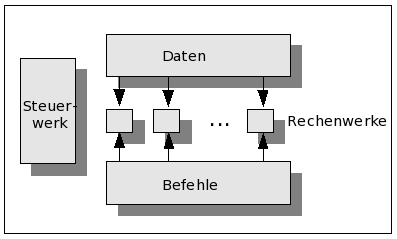
\includegraphics[width=\textwidth]{images/harvard_architektur.png}
  Boris Jakubaschk, \url{https://www.homecomputermuseum.de/technik/rechnerarchitektur/harvard-architektur/}, zuletz aufgerufen am: 19.06.2023
  % TODO: https://en.wikipedia.org/wiki/Cache_hierarchy (Quelle, Grafiken)
\end{example}

\begin{defi}[Cache]{Zugriffszeit}
  Durch die Aufteilung des L1-Cache in Daten- und Instruktions-Cache (Harvard-Architektur) können bei Pipeline-basierten Rechnern gleichzeitig neue Instruktionen zum Füllen der Pipeline geholt werden und bei der Bearbeitung der Operanden die Daten ausgelesen werden.

  Die \emph{Zugriffszeit} $t_Z$ eines Caches kann wie folgt definiert werden:
  \[
    t_Z = t_{C} + (1 - h) \cdot t_{M}
  \]
  Dabei ist $t_C$ die Zugriffszeit des Prozessors für Werte aus dem Cache, $t_M$ die für Daten aus dem Memory und $h$ die Hit-Rate.

  Wenn die Hit-Rate groß sein soll, sind sowohl ein Programm mit hoher räumlicher und zeitlicher Lokalität, sowie ein großer Cache (meist L1, L2 und L3) erforderlich.
\end{defi}

\begin{defi}{Direct Mapped Cache}
  % TODO: https://en.wikipedia.org/wiki/Cache_placement_policies#Direct-mapped_cache (Quelle)
  Bei einem \emph{Direct Mapped Cache} wird der Hauptspeicher in mehreren disjunkte Untermengen organisiert, wobei pro Untermenge genau eine Cache-Zeile definiert ist.

  Platzieren eines Speicherblocks im Cache:
  \begin{itemize}
    \item Bestimmen der Zeilenadresse im Cache, basierend auf Adresse um Hauptspeicher
    \item Speicherblock wird entsprechend im Cache gespeichert, als Tag wird die Hauptspeicheradresse verwendet
    \item vorher gespeicherte Daten werden überschrieben
  \end{itemize}

  Suchen im Cache:
  \begin{itemize}
    \item Bestimmen der Zeilenadresse im Cache, basierend auf Adresse um Hauptspeicher
    \item Tags (Hauptspeicheradressen) werden verglichen
    \item bei gleichen Tags \emph{Cache-Hit}, sonst \emph{Cache-Miss}
    \item bei einem \emph{Cache-Miss} muss der Speicherblock in Cache geladen werden
  \end{itemize}

  Vorteile des Direct Mapped Cache sind, dass nicht alle Adressen im Cache durchsucht werden müssen und das Vorgehen sehr simpel ist.

  Da allerdings pro Untermenge im Hauptspeicher nur eine Zeile im Cache definiert ist, ist die Hit-Rate geringer als bei Alternativen.

  \centering
  % TODO: https://diveintosystems.org/book/C11-MemHierarchy/caching.html (Quelle)
  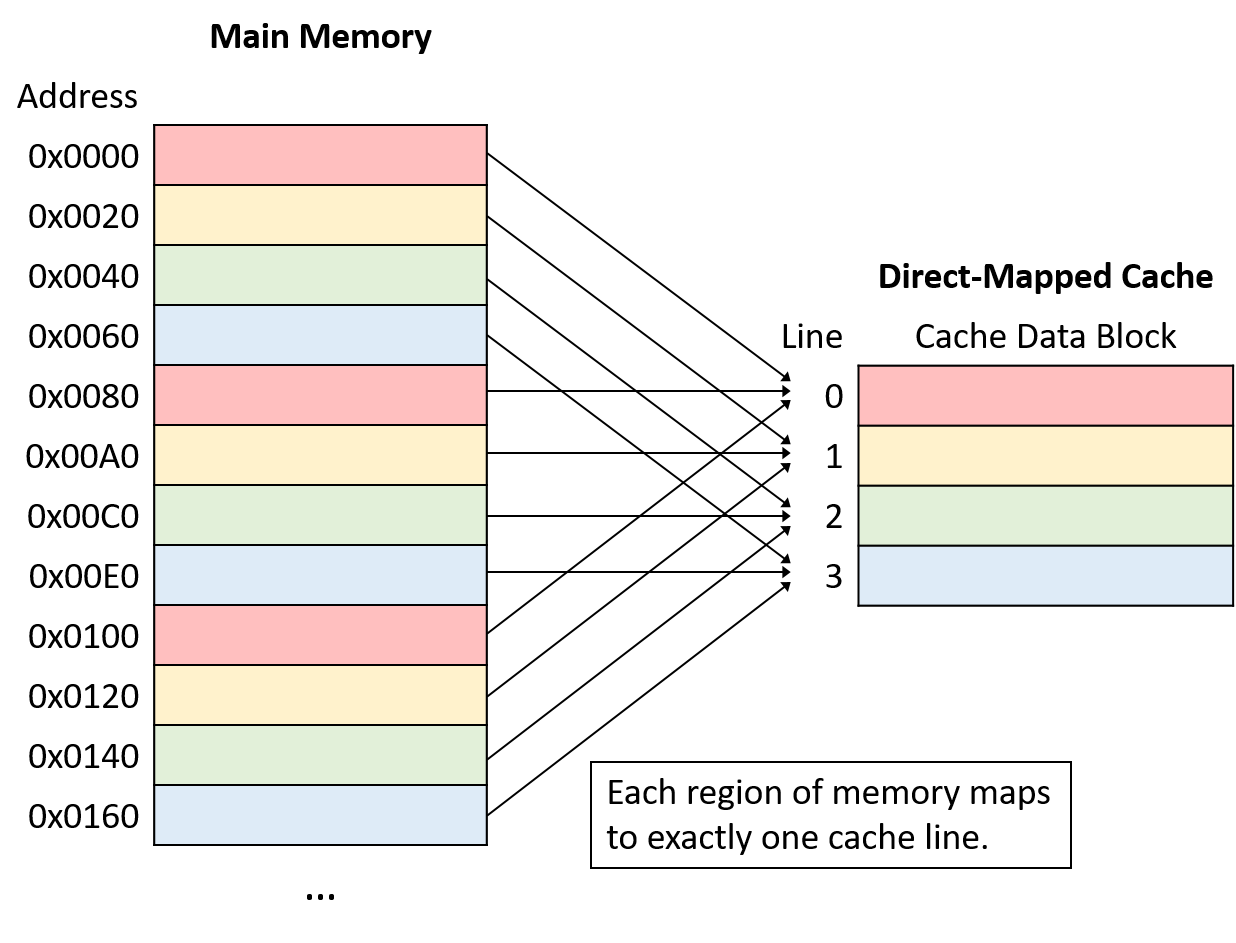
\includegraphics[width=.6\linewidth]{images/direct_mapped_cache.png}
  % 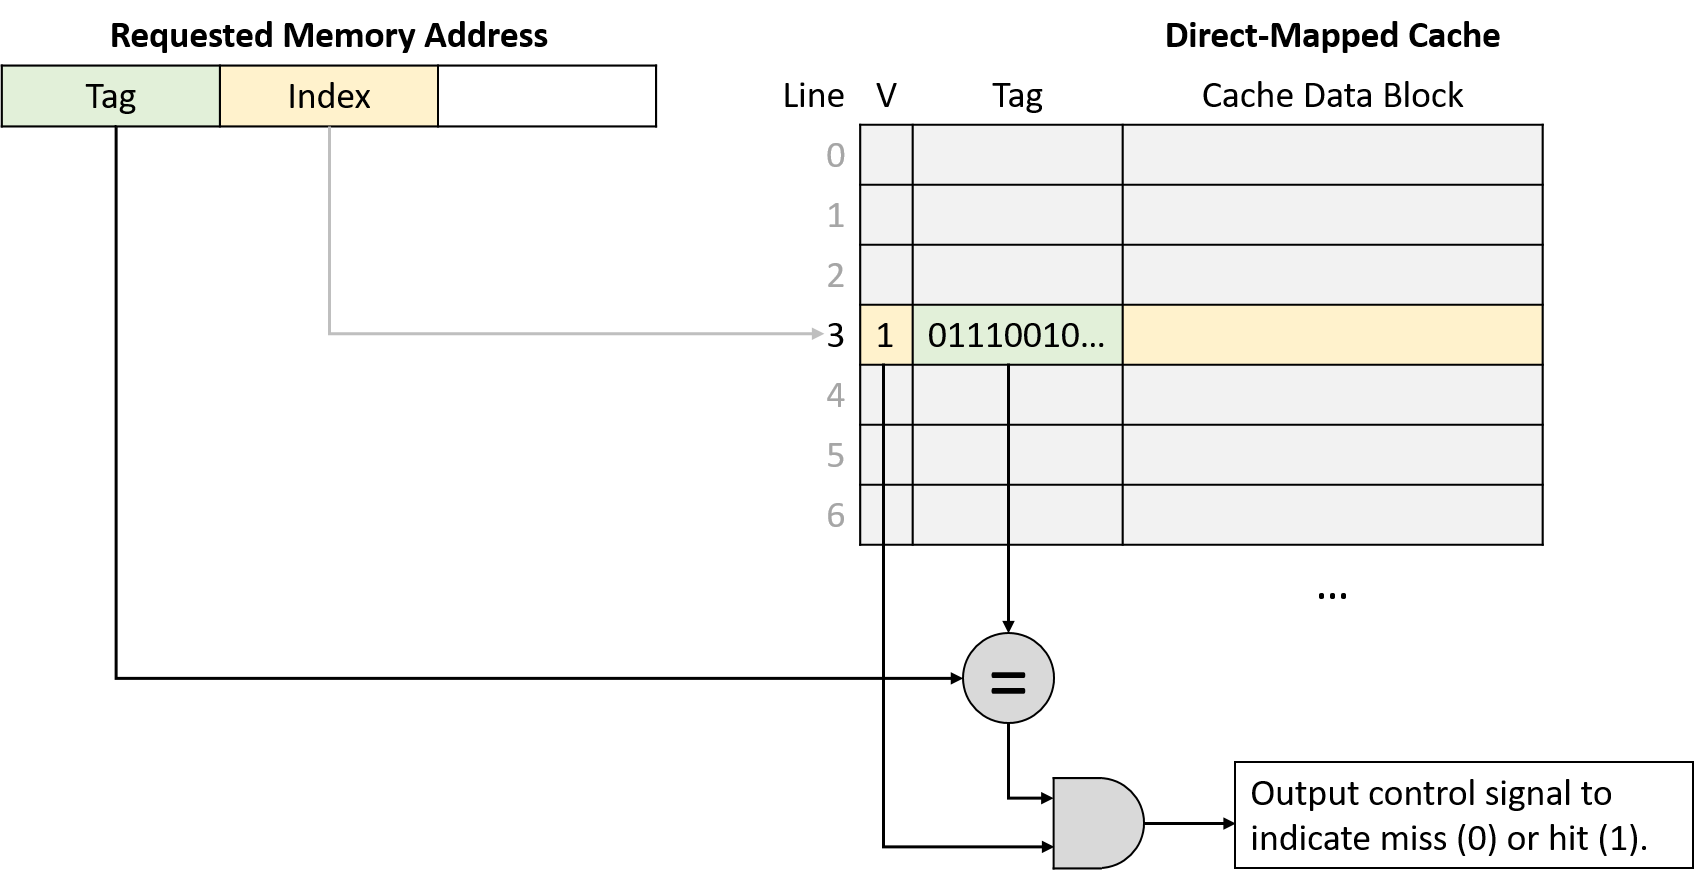
\includegraphics[width=.9\linewidth]{images/direct_mapped_cache_request.png}
\end{defi}

\begin{defi}{N-way Set Associative Cache}


  % TODO: https://diveintosystems.org/book/C11-MemHierarchy/caching.html (Quelle)
  \centering
  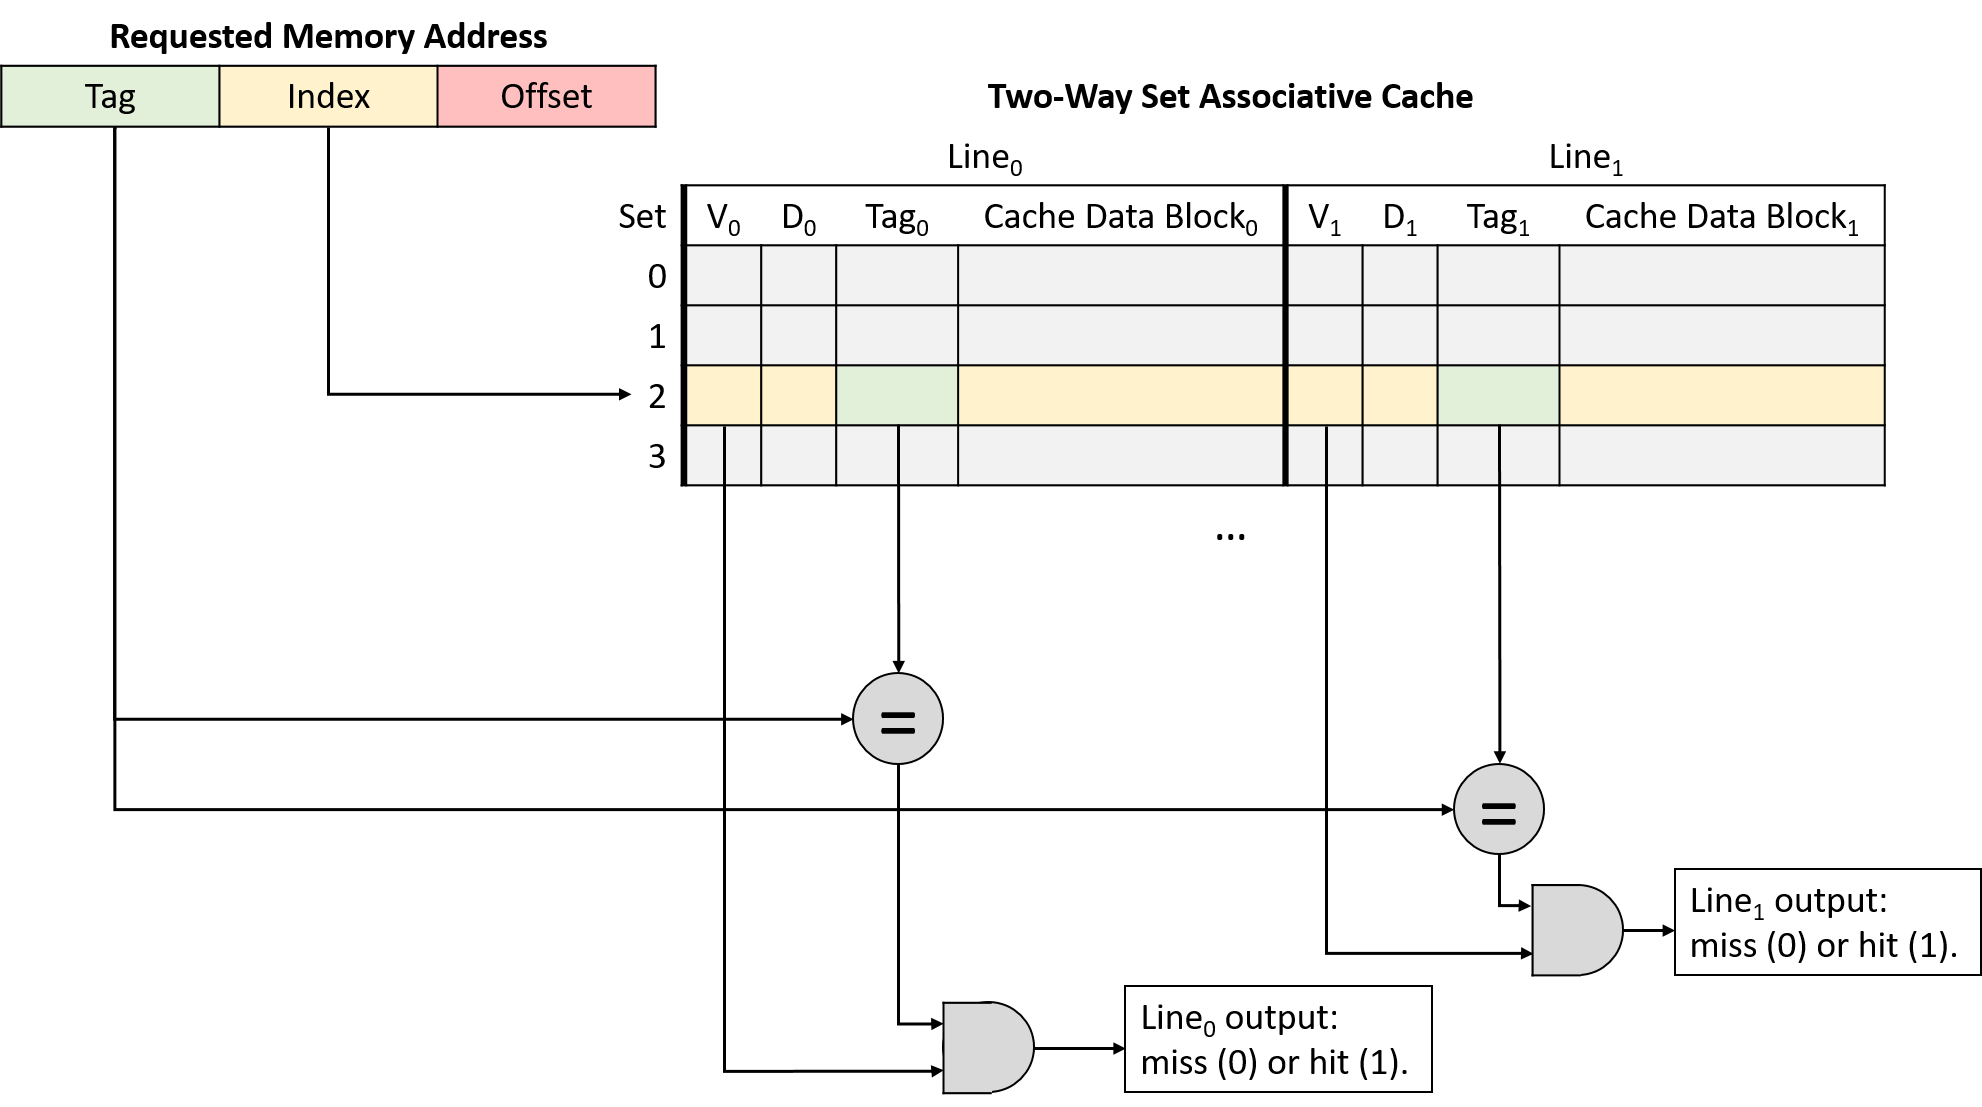
\includegraphics[width=.9\linewidth]{images/2-way_set_associative_cache_request.png}
\end{defi}

\begin{example}[N-way Set Associative Cache]{2-way Set Associative Cache}
\end{example}

\begin{defi}{Fully Associative Cache}

\end{defi}

\begin{defi}{Ersetzungsstrategie}
  \begin{itemize}
    \item Trivial für Direct Mapped Cache
    \item Bei Set Associative oder Fully Associative:
          \begin{itemize}
            \item Random
            \item LRU (Least Recently Used) bzw. FIFO
          \end{itemize}
  \end{itemize}
  Zurückschreiben von Daten:
  \begin{itemize}
    \item \underline{Write through:} Die Information wird sowohl in den Cache als auch ins
          Memory zurückgeschrieben.
    \item \underline{Write back:} Die Information wird nur in den Cache geschrieben. Die
          veränderte Zeile wird erst dann ins Memory geschrieben, wenn die
          Cache-Zeile mit Daten aus anderen Hauptspeicheradressen
          überschrieben werden soll.
          \begin{itemize}
            \item \underline{Vorteil:} Mehrfaches Ändern eines Wertes wird nur im Cache durchgeführt.
            \item \underline{Nachteil:} Ein Read-Miss kann zu einem Schreiben ins Memory führen.
          \end{itemize}
  \end{itemize}
\end{defi}

\begin{bonus}[Cache]{IBM Power 4}

\end{bonus}

\begin{bonus}[Cache]{Intel Itanium}

\end{bonus}

\begin{defi}{Cache Miss}
  Ist keine Kopie der Hauptspeicherzelle a im Cache abgelegt, so
  \begin{itemize}
    \item greift die CPU auf den Arbeitsspeicher zu,
    \item lädt das Datum in den Cache und
    \item lädt das Datum gleichzeitig in die CPU.
  \end{itemize}
\end{defi}

\begin{defi}{Reduzierung der Cache Miss Rate}
  \begin{itemize}
    \item \underline{Cold start miss:} Tritt auf beim ersten Zugriff auf einen Block nach dem Start des Programms oder dem Task-Wechsel (auch bei unendlich großem Cache)
    \item \underline{Capacity miss:} Tritt auf, wenn der Cache nicht alle Blocks speichern kann, die bei der Ausführung durch die CPU benötigt werden (nur bei fully associative Cache)
    \item \underline{Conflict miss:} Tritt auf, wenn ein Block ersetzt werden muß, der anschließend wieder benötigt wird (bei N-way associative Cache)
    \item \underline{Coherence miss:} bei Mehrprozessorsystemen → wird später erklärt
  \end{itemize}
\end{defi}

\begin{defi}[Reduzierung der Cache Miss Rate]{Programmierstrategien}
  Verbessern der Speicherlokalität durch
  \begin{itemize}[\ldots]
    \item Datenstrukturierung
    \item Ändern der Indexierung
    \item Schleifenfusion
    \item Bildung von Teilblöcken
  \end{itemize}
\end{defi}

\begin{defi}{Table-Look-Aside Buffer}
  Bei Rechnern mit virtueller Speicherverwaltung arbeitet der Prozessor mit virtuellen Adressen,
  die durch den TLB in reale Adressen umgesetzt werden.
\end{defi}

\subsection{Entwicklungslinien der Prozessoren}\label{subsec:entwicklungslinien-der-prozessoren}

\begin{defi}{Complex Instruction Set Computer (CISC)}
  Befehls-Code ist Index auf Zeiger-Array für Mikroprogramm,
  die Hardware führt die Sequenz der Mikrobefehle aus.
\end{defi}

\begin{defi}{Reduced Instruction Set Computer (RISC)}
  Der Compiler erzeugt direkt \enquote{Mikrobefehle}.
  Es muss zwar mehr Code erzeugt werden,
  aber die Hardware wird einfacher und damit auch schneller.
\end{defi}

\begin{defi}{Very Long Instruction Word (VLIW)}
\end{defi}

\begin{defi}{Explicitly Parallel Instruction Computing (EPIC)}
  Von HP und Intel wurde 1998/99 die Prozessorarchitektur EPIC entworfen
  und mit dem Intel Itanium ein erster Prozessor realisiert.
  Die Intel-Version der Architektur wird IA-64 (64 bit) genannt.

  EPIC ist die moderne Weiterentwicklung des Konzepts des VLIW.

  Hierbei versucht der Compiler,
  möglichst viele voneinander unabhängige Instruktionen in einer Sequenz zusammenzustellen.
  Er kann dabei durch Umstellen der Befehle die Reihenfolge innerhalb der Sequenz verändern.
  Dies darf aber nicht zu anderen Ergebnissen führen!

  Eine solche Sequenz nennt Intel ein \enquote{bundle}.
\end{defi}

\subsection{Aufgaben}

\aufgabe[Caches]{Ersetzungsstrategie}
{
  Welche Ersetzungsstrategien bei Konflikten können beim Set Associative oder Fully Associative Cache eingesetzt werden?
}
{
  Es können die Ersetzungsstrategien \enquote{Random},
  \enquote{Last Recently Used (LRU)} oder \enquote{First In First Out (FIFO)} eingesetzt werden.
}

\aufgabe[Caches]{Write-Back Cache}
{
  Welchen Vorteil bietet ein Write Back Cache?
}
{
  Mehrfaches Ändern eines Wertes wird nur im Cache durchgeführt.
}

\aufgabe[Cache]{Cache-Miss}
{
  Nennen und erklären Sie vier verschiedene Typen eines Cache-Miss.
}
{
  Es existieren folgende Typen eines Cache-Miss:\\
  \begin{tabularx}{\textwidth}{|l|X|}
    \toprule
    Typ              & Erklärung                                                                                                                                          \\
    \midrule
    Cold start miss: & Tritt auf beim ersten Zugriff auf einen Block nach dem Start des Programms oder dem Task-Wechsel (auch bei unendlich großem Cache)                 \\
    \midrule
    Capacity miss:   & Tritt auf, wenn der Cache nicht alle Blocks speichern kann, die bei der Ausführung durch die CPU benötigt werden (nur bei fully associative Cache) \\
    \midrule
    Conflict miss:   & Tritt auf, wenn ein Block ersetzt werden muss, der anschließend wieder benötigt wird (bei N-way associative Cache)                                 \\
    \midrule
    Coherence miss:  & Tritt in einem mehrprozessorfähigen Cache auf,
    wenn ein Prozessor eine Adresse in den Cache schreibt und ein anderer Prozessor auf die gleiche Adresse zugreifen möchte,
    bevor die Änderungen in den Hauptspeicher geschrieben wurden.                                                                                                         \\
    \bottomrule
  \end{tabularx}
}

\aufgabe[Cache]{Virtuelle Adressen}
{
  Im Cache befinden sich stets reale Adressen.
  Wie heißt der \enquote{Cache} für virtuelle Adressen?
}
{
  Der \enquote{Cache} für virtuelle Adressen heißt \enquote{Translation Lookaside Buffer (TLB)}.
}

\aufgabe[Parallelität]{Risiken}
{
  Nennen und erklären Sie drei Risiken,
  die beim ILP zum Abreißen der gleichmäßigen Instruktionsbearbeitung führen können.
}
{
  \begin{tabularx}{\textwidth}{|l|X|}
    \toprule
    Risiko              & Erklärung                                                                                                           \\
    \midrule
    Structural hazards: & Die HW kann nicht eine bestimmte Aufeinanderfolge von Instruktionen ausführen.                                      \\
    \midrule
    Data hazards:       & Instruktionen hängen vom Ergebnis vorheriger Schritte ab,
    die noch nicht die Pipeline verlassen haben.                                                                                              \\
    \midrule
    Control hazards:    & Zwischen dem \enquote{fetch} von Instruktionen und dem Ändern des Kontrollflusses (branch) entstehen Verzögerungen. \\
    \bottomrule
  \end{tabularx}
}

\aufgabe[]{Prozessoren}
{
  Nennen Sie drei Methoden,
  die im Itanium Prozessor eingesetzt werden,
  um Instruktionen beschleunigt abarbeiten zu können.
}
{
  \begin{itemize}
    \item Predication
    \item Data Speculation
    \item Control Speculation
  \end{itemize}
}